\section{Exploración Univariada}\label{univariada}


El Programa de Naciones Unidas para el Desarrollo (PNUD) señala que Colombia tiene un alto desarrollo humano. El país ocupa el puesto 91 entre 186, en un informe que evalúa los logros de las naciones en educación y salud, y la disponibilidad de recursos para ofrecerles a sus habitantes un nivel de vida digno.

En el Índice de Desarrollo Humano (IDH) en América Latina, Colombia se ubica en la casilla número 12, muy por debajo de Chile, Argentina, Uruguay y Cuba. Sólo supera a naciones como El Salvador, Guatemala y Bolivia. Según el informe en nuestro país los niños estudian en promedio 7,3 años, mientras el “período esperado de escolaridad” son 13,6.


% Table created by stargazer v.5.2.2 by Marek Hlavac, Harvard University. E-mail: hlavac at fas.harvard.edu
% Date and time: jue., jul. 05, 2018 - 11:33:22 a.m.
\begin{table}[!htbp] \centering 
  \caption{Medidas estadísticas} 
  \label{stats} 
\begin{tabular}{@{\extracolsep{5pt}}lccc} 
\\[-1.8ex]\hline 
\hline \\[-1.8ex] 
Statistic & \multicolumn{1}{c}{Mean} & \multicolumn{1}{c}{Median} & \multicolumn{1}{c}{St. Dev.} \\ 
\hline \\[-1.8ex] 
IDH & 0.802 & 0.804 & 0.042 \\ 
Poblacion.Cabecera & 1,196,730.000 & 717,197 & 1,982,287.000 \\ 
Poblacion.Resto & 360,590.300 & 268,111.5 & 331,887.600 \\ 
Poblacion.Total & 1,557,320.000 & 1,028,429 & 2,202,522.000 \\ 
\hline \\[-1.8ex] 
\end{tabular} 
\end{table} 
La población de Colombia se concentra en las áreas andinas y en la costa del Atlántico, donde se aprecian los núcleos demográficos de la sabana de Bogotá, conformado por Bogotá y Soacha, del valle de Aburrá, que comprende a Medellín, Bello e Itagüí, del Valle del Cauca, compuesto por Cali y Palmira. Lo mismo que las ciudades de la Costa Atlántica, Cartagena, Barranquilla y Santa Marta. Al igual que los centros demográficos de Bucaramanga y Cúcuta en la zona de los Santanderes, el Eje cafetero, Huila y Tolima.

Lo mismo que las ciudades de la Costa Atlántica, Cartagena, Barranquilla y Santa Marta. Al igual que los centros demográficos de Bucaramanga y Cúcuta en la zona de los Santanderes, el Eje cafetero, Huila y Tolima.

\begin{figure}[h]
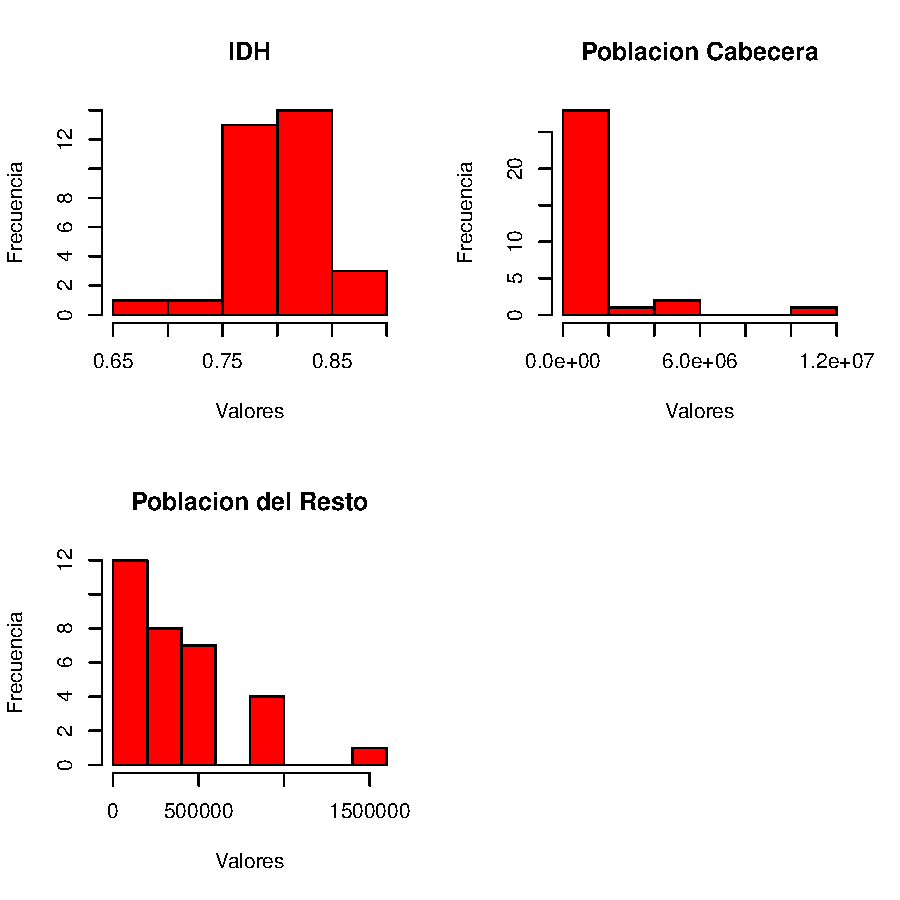
\includegraphics{univariada-hist}
\caption{Distribución de Indicadores}
\label{hist}
\end{figure}

Esta concepción requiere que la medición del nivel de desarrollo humano de un determinado país, comunidad o grupo social, no se base solamente en componentes económicos que, aunque también son importantes considerar, constituyen una aproximación incompleta dado la complejidad del proceso señalado. Dentro del esquema propuesto por el PNUD se procura enfatizar en la gran divergencia existente entre niveles de riqueza material y de desarrollo humano. Por esta razón, el principal objetivo subyacente en la construcción del IDH es proporcionar referencias cuantitativas de las privaciones humanas y de las distancias existentes con respecto a metas posibles de alcanzar y monitorear la eficacia de las políticas en curso. 


\begin{figure}[h]
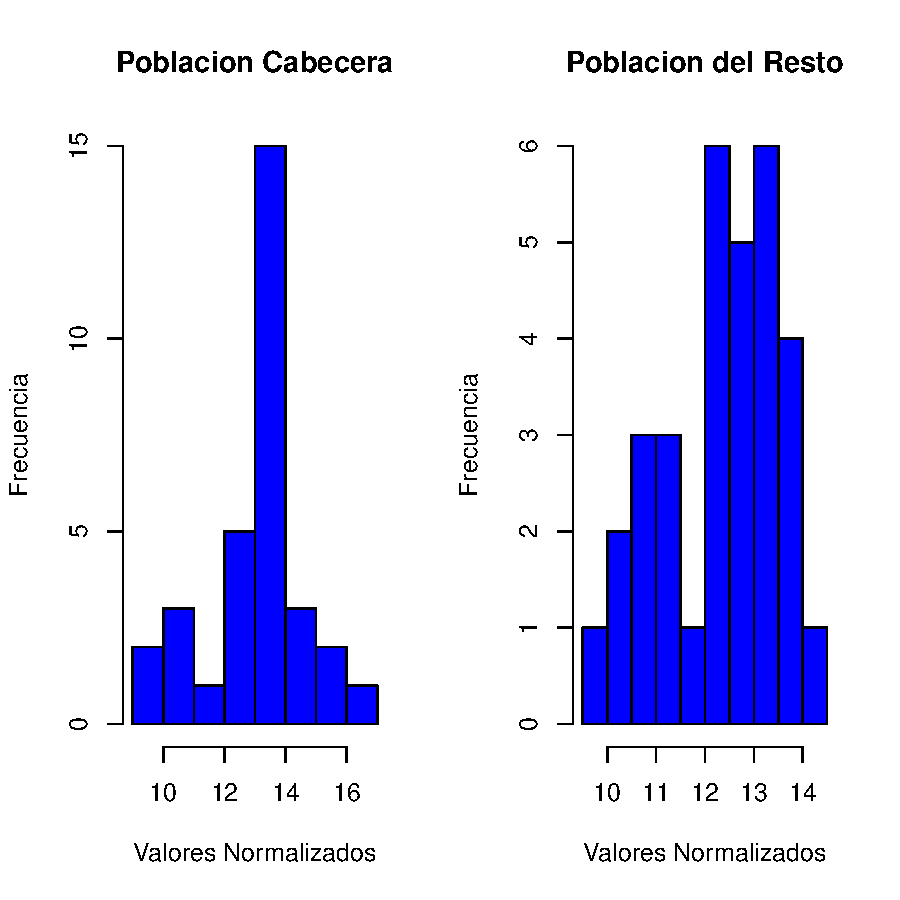
\includegraphics{univariada-hist1}
\caption{Distribuciòn de Indicadores de Poblaciones Normalizado}
\label{hist1}
\end{figure}

Precisamente, en este trabajo se intenta realizar una descripción basada en la síntesis de los tres aspectos esenciales mencionados, motivados especialmente por cierta paradoja estadística que explicamos a continuación: desde que el PNUD iniciara el cálculo del IDH en 1990, Argentina se encuentra en el grupo de países con desarrollo humano ALTO, aunque su posición en el ránking mundial fue variando desde el puesto 43 en 1991 al Nº 30 en 1996 y al lugar Nº 39 en 1999, a tal punto de figurar entre los primeros puestos en el conjunto de países latinoamericanos. Pero, al tratarse de un promedio nacional, el indicador oculta importantes diferencias en la distribución regional y provincial de los distintos aspectos del desarrollo humano y por lo tanto merece que nos ocupemos de observar la situación real de las provincias y en forma particular de las que forman el Nordeste Colombianob segun \cite{konrad-adenauer-stiftung_indice_2003} . 

\endinput
